\section{Problem 3}

{\bfseries 3.1 Part 1}

We have conducted a series of experimentation with the simple data from Bishop's Figure 1.4. For M = 0, it should be a horizontal line regardless of the lambda because w0 is not being penalized.  As M increases, the curve is more likely to overfit the data. For M = 1,3, increasing the lambda reduces the quality of the models because the original models  match the data well. For M = 9, the original unregularized model overfits the data. As we increase lambda, the model becomes more similar to the sin2pi model. This shows that using regularizatio helps alleviates the overfitting problem. 

\begin{figure}[!htb]
\minipage{0.32\textwidth}
  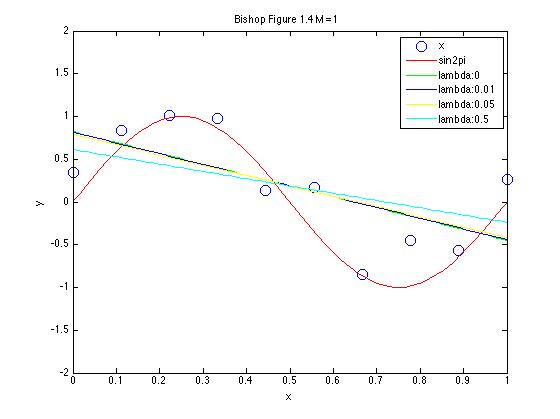
\includegraphics[width=\linewidth]{figures/p3_bishop_m=1}
  \caption{M = 1}\label{fig:figures/p3_bishop_m=1}
\endminipage\hfill
\minipage{0.32\textwidth}
  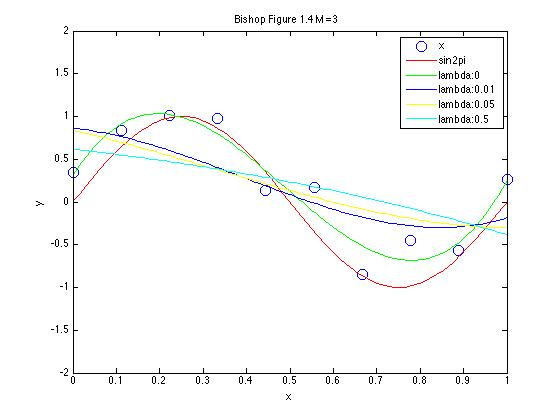
\includegraphics[width=\linewidth]{figures/p3_bishop_m=3}
  \caption{M = 3}\label{fig:figures/p3_bishop_m=3}
\endminipage\hfill
\minipage{0.32\textwidth}%
  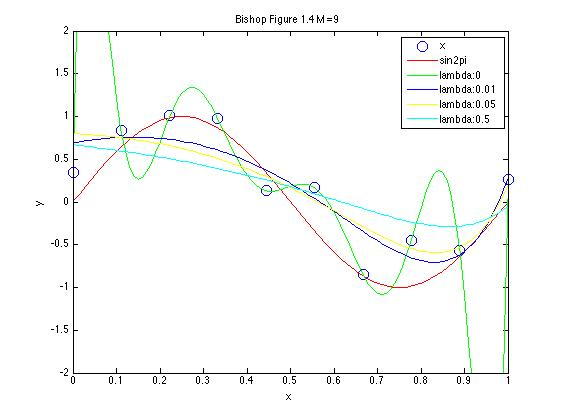
\includegraphics[width=\linewidth]{figures/p3_bishop_m=9}
  \caption{M = 9}\label{fig:figures/p3_bishop_m=9}
\endminipage\hfill
\end{figure}

{\bfseries 3.2 Part 2}

We selected M=1,4,6 with varying lambdas and plotted the error on the validation set in the figures below. We have splitted a separate test set from the validation set for evaluating the best model selected. 
First, comparing figure~\ref{fig:p3_regressB_m=2} to~\ref{fig:p3_regressA_m=6} with figure~\ref{fig:p3_regressA_m=2} to~\ref{fig:p3_regressB_m=6}, we can see that in general error from training set B is higher than that from training set A. This is because there is a outlier in trainng set B, as shown in Figure~\ref{fig:p3_training_validation_data}. This prevented us from creating a good model. 

\begin{figure}[!htb]
\minipage{0.32\textwidth}
  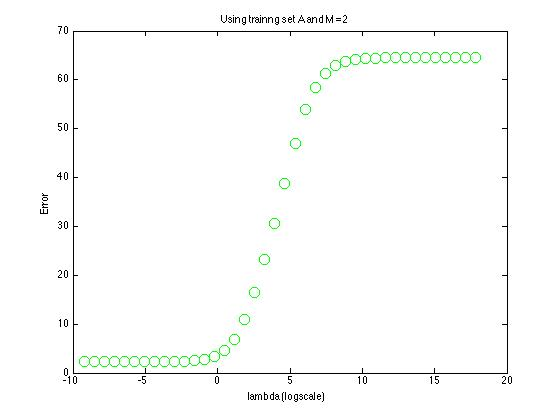
\includegraphics[width=\linewidth]{figures/p3_regressA_m=2}
  \caption{Set A, M = 2}\label{fig:p3_regressA_m=2}
\endminipage\hfill
\minipage{0.32\textwidth}
  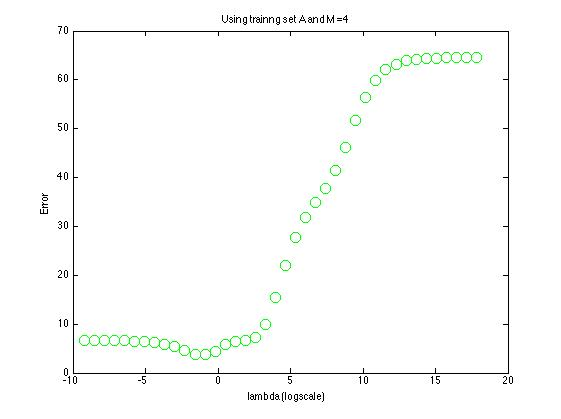
\includegraphics[width=\linewidth]{figures/p3_regressA_m=4}
  \caption{Set A, M = 4}\label{fig:p3_regressA_m=4}
\endminipage\hfill
\minipage{0.32\textwidth}%
  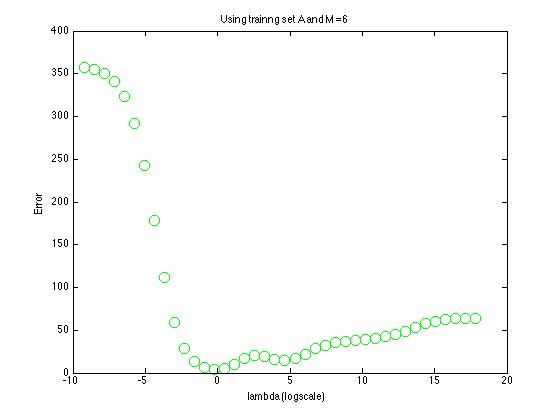
\includegraphics[width=\linewidth]{figures/p3_regressA_m=6}
  \caption{Set A, M = 6}\label{fig:p3_regressA_m=6}
\endminipage
\end{figure}


\begin{figure}[!htb]
\minipage{0.32\textwidth}
  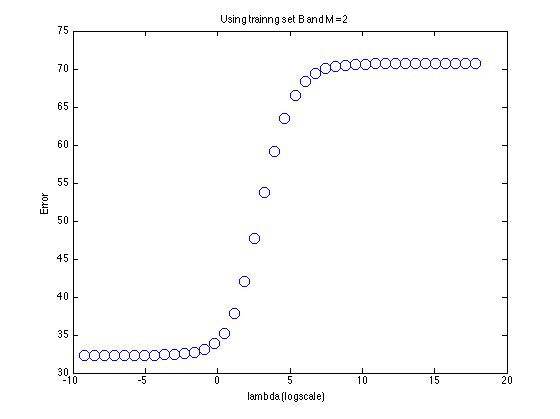
\includegraphics[width=\linewidth]{figures/p3_regressB_m=2}
  \caption{Set B, M = 2}\label{fig:p3_regressB_m=2}
\endminipage\hfill
\minipage{0.32\textwidth}
  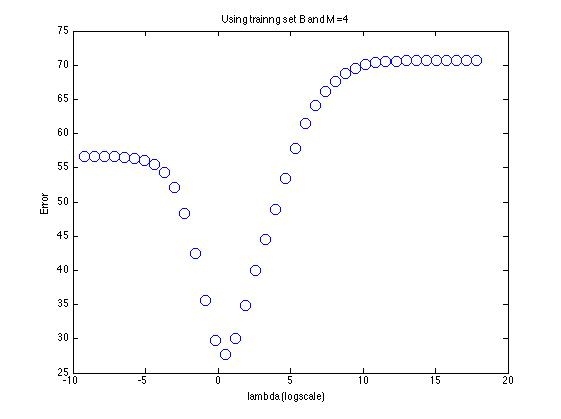
\includegraphics[width=\linewidth]{figures/p3_regressB_m=4}
  \caption{Set B, M = 4}\label{fig:p3_regressB_m=4}
\endminipage\hfill
\minipage{0.32\textwidth}%
  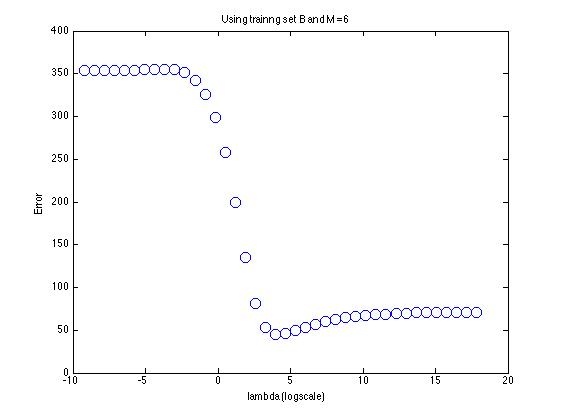
\includegraphics[width=\linewidth]{figures/p3_regressB_m=6}
  \caption{Set B, M = 6}\label{fig:p3_regressB_m=6}
\endminipage
\end{figure}


The best configurtion from the model in A is with M = 2 with lambda = 0.01(figure~\ref{fig:p3_regressA_m=2}). For M = 2, the error is alredy very small wihtout regularization. Increasing the lambda gradually increases the validation error because it leads the model away from the data observed. As we incrase M, the error incrases as the model overfits the original traning A data. For M = 6, the model has significantly higher error on the validation set as shown in figure~\ref{fig:p3_regressA_m=6}.  However, we 
can see the effect of regularing the weight. The error rate decreases as we increase the size of lambda. However, after the minimum point(lambda close to 1), the error goes up again as the weight factors are no longer guided by the training data set. 

For training data B, we can see the error with lambda = 0 is much larger compare to A. This is because there is an outlier in the traning data B. Since the model overfits the data, regularization is important for using training set B. We can see a clear point of change (0 and 3) in figure~\ref{fig:p3_regressB_m=4} and~\ref{fig:p3_regressB_m=6}. The validation error decreases before the point and increases afterwards. 

%TODO: write a little bit about what are the errors on the testing set.
We tested the best model and lambda pair on the test set and the error we observed is comparable to that on the validation set. 

{\bfseries 3.3 Part3}
\begin{figure}[!htb]
  \minipage{0.48\textwidth}
  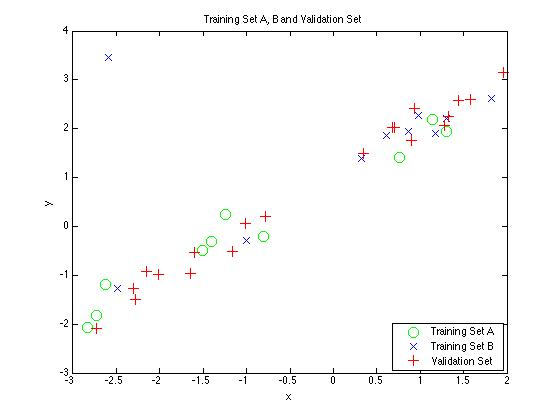
\includegraphics[width=\linewidth]{figures/p3_training_validation_data}
  \caption{Training and Validation Data}\label{fig:p3_training_validation_data}
  \endminipage\hfill
  \minipage{0.48\textwidth}%
  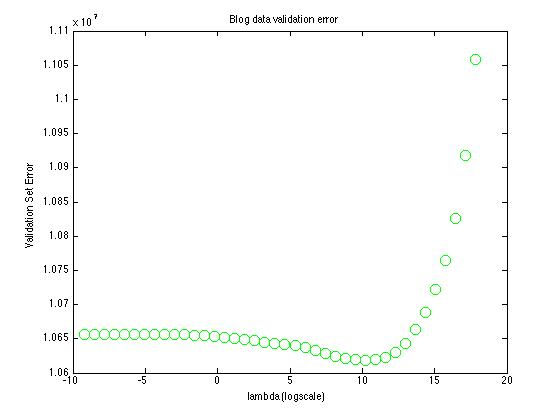
\includegraphics[width=\linewidth]{figures/p3_blogdata_lambda}
  \caption{Blog validation data error}\label{fig:p3_blog_data}
  \endminipage\hfill
\end{figure}

Figure~\ref{fig:p3_blog_data} shows that as we increase lambda, the error first decreases. However, as we futher increase lambda, the weight vectors no longer rely on the data, the error increases quickly. Even with the best lambda we chose from the validation set, the error for the test set is still large
in the order of $10^{7}$. However, we belive that this is because the simple linear model (without non-linear basis functions) is unable to accurately describe a model. 
